% 中文阅读译稿；对应 chapters/07-evaluation.tex，不增加实验或结论。
\chapter{实验评估与研究发现}
\label{ch:evaluation}
\chaptermark{实验评估}

本章通过构建测量、受控执行改动、留出查询预算选择和跨系统搜索，回答论文的四个研究问题。对于\textbf{RQ1}（构建与容量），最大被测索引在单卡上搜索 17.78 百万个向量，常驻设备显存为 20.44\,GiB；对应的冷训练加添加记录为 10.40\,s。对于\textbf{RQ2}（正确且高效的 GPU 执行），两组查找表在 22/24 个配置中领先；批大小 8 时，调度扫描的吞吐量几何平均提高至 $2.727\times$，并保持被测最终标识符集合一致。对于\textbf{RQ3}（预算质量与净成本），所选配置的平均 QPS 在 10/12 个单元中优于固定 $\alpha=100$，在 9/12 个单元中优于固定 $\alpha=64$，但最多 40/64 次校准抽样超过相对 oracle 的召回率损失阈值。对于\textbf{RQ4}（竞争区间），召回率 0.97 处，插值比较中 JHQ 在三个 E1 数据集上最快，在 arXiv 上与 IVF-RaBitQ 数值接近；CAGRA int8 则在较低召回率领先。

\section{最终实验清单与对照实验组}
\label{sec:7-1}

实验分组区分了回答 RQ1--RQ4 所需的证据。组件名称描述机制，版本号标识实现来源。记录中的运行源码版本、二进制名称以及源码到结果的映射见\cref{app:reproducibility}。

\subsection{证据分组与测量边界}

\Cref{tab:7-manifest} 列出了本章使用的实验组。版本号表示不同的实验实现，而不是对同一个不变基准的连续测量。尤其需要区分历史 ADC 论文与后来的 v69/v71 实验：它们的计时结果不同。本章相应的数字以较新的原始记录为准；历史打包访存和精排实验则作为独立消融保留。将这些实验的加速比直接相乘，会混合不同基线，得不到实际测量过的系统加速比。

\begin{table}[tbp]
\centering
\caption{实验与证据分组。数量表示测量配置或检查次数，不代表独立索引构建次数。所有实验均使用 RTX 5090，但计时协议有所不同。}
\label{tab:7-manifest}
\small
\begin{tabularx}{\linewidth}{@{}lXl@{}}
\toprule
实验组 & 目的与实现 & 覆盖范围 \\
\midrule
E1 & v69 与 cuVS 图索引、PQ、RaBitQ、暴力搜索比较 & 1,590 个点；4 个数据集 \\
LUT & v71 查找表分组，$\glut\in\{1,2,4,8\}$ & 24 个单元；96 个变体 \\
打包访存 & 历史字节/机器字访存析因对照 & 48 个配对单元 \\
精排 & v61 标量、加载方式与 lane 数消融 & 13 个配置 \\
扫描/共享界 & v62 全局选择；v63 共享界 & 64 / 48 个正确性比较 \\
调度 & 集成后的 v65 执行策略 & 50 个工作负载—批大小单元 \\
探针选择 & v69 精确 FP32 探针选择 & 1,792 个合成用例 \\
预算 & v69 抽样、全校准池与 oracle 预算 & 12 个单元；每个 $S$ 抽样 64 次 \\
规模 & v69 搜索、冷构建与常驻显存 & BGE 与 Stella 扩展实验 \\
\bottomrule
\end{tabularx}
\end{table}

E1 的环境记录为 NVIDIA GeForce RTX 5090，设备报告显存 32,607\,MiB，驱动 595.71.05，CUDA 13.0，cuVS 26.08.01。容器的 CPU 配额为 25 核，OpenMP 限制为 16 个线程。JHQ 使用 Release 构建，先编译为 compute\_80 PTX，再由驱动针对设备即时编译；基线使用已安装的原生 cuVS 库。

跨系统比较的主要计时边界为“主机输入到主机输出”：从主机内存中的 FP32 查询开始，到 top-10 标识符和距离返回主机内存、流同步完成为止。它包含数据传输、查询预处理与搜索；CAGRA int8 的查询量化也包含在内。基线复用资源句柄和输出缓冲区。E1 使用五轮计时，每轮通常调用 24 次。当包含首次调用的预热区间超过每次调用的阈值时，基线程序减少调用次数；274 个点采用了较少调用，其中也包括稳态速度较快的点。报告的 QPS 是各轮吞吐量的中位数，每轮吞吐量由总查询数除以总耗时得到，而不是单次调用延迟中位数的倒数。预热、索引构建以及任何预算校准均不计入。基线的纯设备端时间仅作为辅助结果：JHQ 没有等价的设备端查询接口，将这些时间混入主要比值会改变比较口径。

\subsection{指标与可复现性}

所有实验均采用平方 L2 距离和 $k=10$。召回率是找回真实 top-10 标识符的平均比例；即使 ground-truth 文件每行存储了更多结果，也只比较前十项。精排系数决定候选保留数 $c=\max\{k,\lceil\alpha k\rceil\}$。本章中，$\glut$ 表示笛卡尔查找表分组数，$\gscan$ 表示并行扫描组数；这两个参数控制不同的工作。

本章分析脚本只读取已有测量，不运行新的 GPU 实验。它核对记录数量与正确性字段，重新计算配对比值和匹配召回率结果，并直接从原始记录生成数字表格。配套证据清单记录了所用文件的 SHA-256 哈希。其中的源码检出版本号表示本次核对所使用的仓库快照，并不意味着所有历史二进制程序都由这个提交构建。各次运行的原始日志头和实验报告仍保留其各自构建来源。这样既能复现当前图表，也不会错误地给历史实验重新标注版本。\footnote{报告仓库提供 \path{scripts/build_ch7.py}、\path{data/ch7/audit.json}、\path{data/ch7/matched.csv} 和证据清单 \path{data/ch7/sources.csv}。脚本需要同级目录中包含归档测量的 \texttt{JHQ\_GPU} 仓库。}

\section{现代 GPU ANN 的召回率—QPS 前沿}
\label{sec:7-2}

本节通过定位共同召回率下的运行区间回答 RQ4，同时包含竞争方法更快的区间。

\subsection{比较范围与前沿构造}

\Cref{fig:7-frontiers} 将 JHQ-GPU 与 CAGRA fp32、经过标量量化的 CAGRA int8、IVF-RaBitQ、IVF-PQ 和 GPU 暴力搜索进行比较。CAGRA 代表图搜索；PQ 和 RaBitQ 代表使用压缩表示的倒排文件方法\cite{cagra,pq,ivfrabitq}。四个数据集分别为 Vogue（$932{,}328\times768$）、arXiv（$2{,}253{,}000\times768$），以及各含 999,000 个向量、维度分别为 1,536 和 3,072 的两个 OpenAI 数据集。每个数据集使用 1,000 条查询，各方法共享同一份 ground-truth 文件。

每种方法贡献其非支配的实测运行点。如果同一方法的另一配置在召回率和吞吐量上均不差、且至少一项严格更好，则该点被剔除。因此，一条前沿组合了不同搜索参数，有时还组合了不同索引配置；它并不一定表示同一个固定索引的变化轨迹。每个数据集上，JHQ 提供 27--39 个测量点，各基线组提供 54--264 个点。E1 解析器得到 1,590 个有效点，没有失败记录，也没有无效标识符或行内重复标识符标记。这个数量表示参数扫描的规模，而不是 1,590 次独立重复实验。

参数覆盖较为充分。CAGRA 改变图出度 32/64、搜索宽度 1--8 和中间 top-$k$ 容量 32--512。RaBitQ 改变 4/8/9-bit 预算、支持的搜索模式以及最高 1,024 的探针数。PQ 改变编码长度、查找精度和探针数。JHQ 同时改变探针数与精排预算，并在初始网格无法充分覆盖召回率时扩展网格。比较结论因而受限于这些已记录的参数网格。某条曲线在目标召回率之前结束，表示该区间没有测量，不能证明该方法无法达到目标。

\begin{figure}[tbp]
\centering
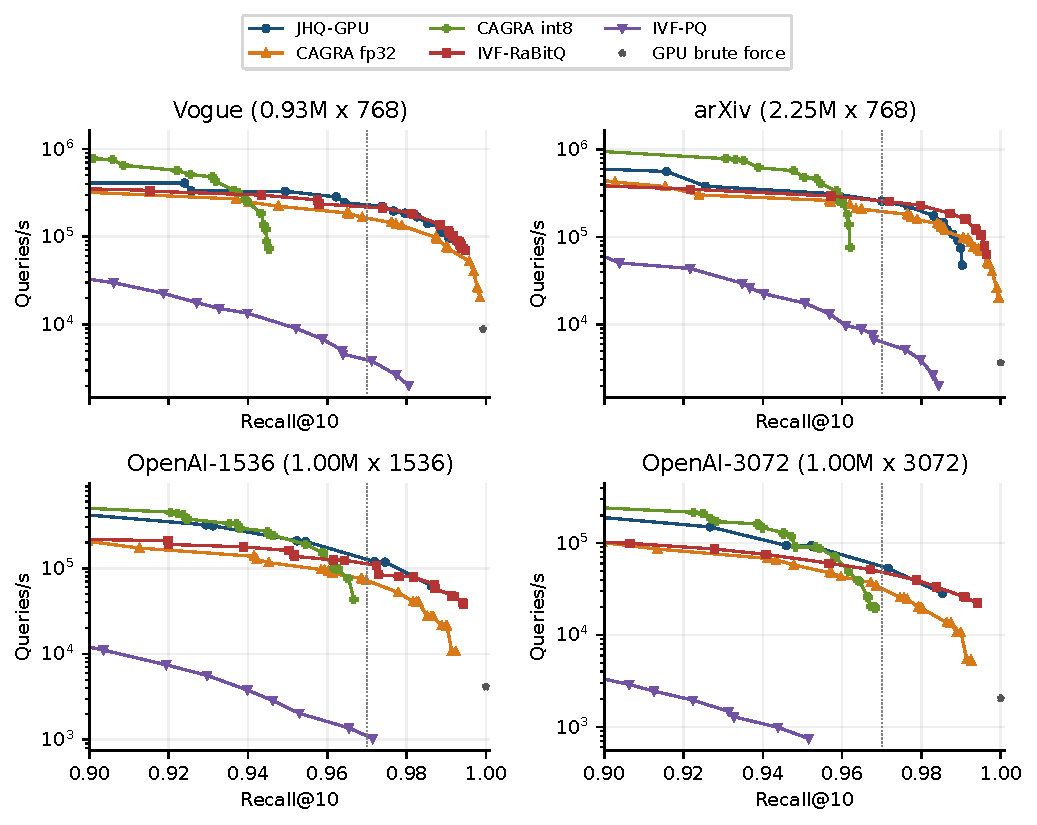
\includegraphics[width=\linewidth]{ch7/frontiers.pdf}
\caption{四个 E1 数据集上实测的主机到主机召回率—QPS 前沿。图中从召回率 0.90 开始显示，并在 0.97 处标出竖线；构造前沿时纳入了包括 CAGRA int8 在内的全部基线组。连线连接实测点，吞吐量轴为对数坐标。}
\label{fig:7-frontiers}
\end{figure}

这些曲线比较的是可达到的吞吐量，而不是相同显存占用下的表现。JHQ 每个向量约存储 $d/8$ 字节主码、$d$ 字节残差码以及元数据。九比特 RaBitQ 的名义编码预算为 $9d/8$ 字节，与 JHQ 接近，但它的 4/8-bit 配置使用更少存储。CAGRA int8 还存储图边；PQ 编码长度可变；CAGRA fp32 保留 FP32 向量。对这些选项取性能包络有助于部署选择，但不能单独证明相同显存预算下的表示优势。显存证据在\cref{sec:7-7}另行讨论。

\subsection{匹配召回率与不同运行区间的反向结果}

\Cref{tab:7-matched} 使用两种估计方式，量化召回率 0.97 附近的表现。插值估计在相邻前沿点之间对吞吐量取对数后进行线性插值，不向覆盖范围之外外推。实测阈值估计选取达到目标召回率的最快采样点。插值估计将与目标相差不超过 $5\times10^{-4}$ 的实测召回率视为匹配；实测阈值估计则要求召回率至少达到目标。插值减小了参数网格间距不一致的影响；实测阈值估计对应真实记录过的配置。两者都不能凭空产生一个召回率恰好等于目标的新测量。

\begin{table}[tbp]
\centering
\caption{召回率 0.97 下的比较。每组比值依次为“插值 / 实测阈值”；大于一表示 JHQ 更快。JHQ kQPS 为插值估计。arXiv 与 RaBitQ 的微小差异随估计方法而改变方向。}
\label{tab:7-matched}
\small\setlength{\tabcolsep}{4pt}
% Generated by scripts/build_zh_tables.py; numeric rows reuse English tables.
\begin{tabular}{@{}lrrr@{}}
\toprule
数据集 & JHQ kQPS & 相对 CAGRA fp32 & 相对 IVF-RaBitQ \\
\midrule
Vogue & 230.8 & 1.416 / 1.537 & 1.059 / 1.046 \\
arXiv & 258.6 & 1.317 / 1.422 & 0.996 / 1.015 \\
OpenAI-1536 & 126.7 & 1.747 / 2.294 & 1.130 / 1.111 \\
OpenAI-3072 & 55.9 & 1.747 / 2.088 & 1.157 / 1.346 \\
\bottomrule
\end{tabular}

\end{table}

相较于 CAGRA fp32，该目标下的插值比值从 arXiv 的 $1.317\times$ 到两个 OpenAI 数据集的 $1.747\times$ 不等。相较于 IVF-RaBitQ，对应数值分别为 $1.059\times$、$0.996\times$、$1.130\times$ 和 $1.157\times$。arXiv 的结果应视为接近平手：插值吞吐量略低，但实测阈值比较略高。如果将其表述为明确获胜，就会让插值约定获得超出测量本身所支持的证据权重。

在有共同覆盖的比较中，目标召回率 0.90--0.985 范围内，JHQ 相对 CAGRA fp32 的插值优势约为 $1.10$--$2.44\times$。但是，加入 CAGRA int8 后，低召回率区间的解释发生变化：在 0.90--0.92 附近，其低精度图搜索可以快于 JHQ。在更高召回率下，IVF-RaBitQ 常重新领先，包括若干 0.98 及以上目标。在 arXiv 约 0.99 的召回率处，记录网格中的 CAGRA fp32 也快于 JHQ。因此，可被证据支持的结论是：JHQ 在部分有价值的区间具有竞争力，尤其是中高召回率附近，而不是全面优于现代 GPU ANN 方法。

CAGRA int8 在 Vogue、arXiv、OpenAI-1536 和 OpenAI-3072 上的最高实测召回率分别为 0.9453、0.9620、0.9667 和 0.9683，因此这些网格中没有达到 0.97 的配置。按相同插值规则，目标召回率 0.90--0.92 处，它约比 JHQ 快 $1.20$--$1.98\times$；在 arXiv 的 0.95 和两个 OpenAI 数据集的 0.94 处也仍然更快。0.97 的结果针对具有测量覆盖的方法，不能推广为低于 0.97 的每个目标均领先。

网格稀疏时，两种估计可能有明显差异。例如，OpenAI-1536 在召回率 0.97 处相对 CAGRA fp32 的比值，插值为 $1.747\times$，而按满足阈值的实测点计算为 $2.294\times$。后一个数值包含了基线下一个超过阈值的测量点所付出的代价，不能将其表述为在完全相同召回率下直接测得的同等幅度优势。配套匹配表保留两种估计，并标明没有覆盖的目标，使读者能够区分真实的运行区间结果与参数采样带来的影响。

\subsection{结果解释与比较限制}

JHQ 将低成本主码筛选与选择性残差访问结合。当只需精排少量已扫描候选时，这为其有竞争力的吞吐量提供了合理解释。后面的内核与预算消融直接检验这一解释的部分环节。仅靠跨系统曲线，不能将收益归因于某个单一组件，因为各方法在路由、表示、预处理、索引构建和软件接口上均有差异。尤其是，数据集维度提高的同时，数据分布与规模也在变化。因此，OpenAI 数据集上更大的比值，并不是“维度提高导致 JHQ 优势扩大”的受控证据。

即便对齐主要计时边界，比较中仍存在限制。JHQ 从 C++ 调用，CAGRA 和 PQ 则通过 Python 绑定调用；即使复用资源，主机端开销仍可能有小幅差异。JHQ 输出回传至可分页主机内存，基线使用页锁定内存。编译目标不同，无关的主机负载也无法完全控制。对于很小的性能差距，这些因素不可忽略。五轮测量描述的是已构建索引上的重复执行，不能估计独立重建索引或换一台机器后的变化。

\section{笛卡尔查找表、打包加载与 lane 协作精排}
\label{sec:7-3}

针对 RQ2，消融区分了保持表示不变的查找表、加载改动与协作式残差评分，并同时测量内核效果和整体应用效果。

\subsection{查找表的精确因子化及其吞吐量影响}

笛卡尔因子化改变的是已表示主码距离的计算方式，而不是重新训练一个量化器。将一个八比特笛卡尔编码拆为两个四比特分量，可把 256 项查找表替换为 $2\times16=32$ 项。对于 FP32 表项，每个对应查找表由 1,024 字节降为 128 字节，即缩小八倍。数学上的评分保持不变，但浮点求值顺序仍可能改变末尾比特。因此，仅凭查找表更小，不能断言完整 ANN 输出逐位一致。

\Cref{fig:7-lut} 比较六个数据集上的笛卡尔查找表分组，探针数为 8/32/128/512、固定 $\alpha=100$，以及 $\glut\in\{1,2,4,8\}$。每个变体有五轮计时；除 Stella 使用 999 条查询外，批大小均为 1,000。在 24 个单元中，两组查找表有 22 个取得最高吞吐量中位数。例外是 arXiv 的 128 探针配置，单组约快 0.23\%；以及 OpenAI-3072 的八探针配置，四组约快 0.84\%。这些小差异更适合视为接近平手。新版统计是 22/24，而不是历史 ADC 论文中的 23/24。

\begin{figure}[tbp]
\centering
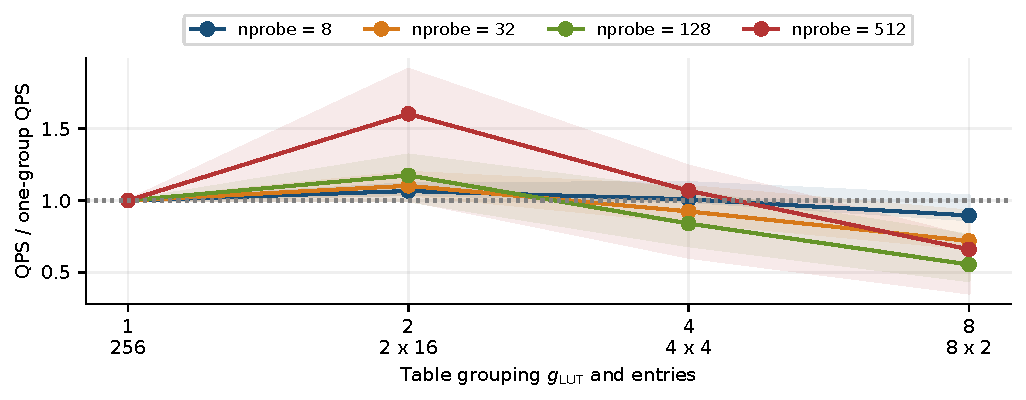
\includegraphics[width=\linewidth]{ch7/lutgroups.pdf}
\caption{固定 $\alpha=100$ 的笛卡尔查找表分组实验（v71）。组数表示 $\glut$，不是并行扫描组数。曲线为各数据集相对单组 QPS 比值的中位数，阴影表示范围。}
\label{fig:7-lut}
\end{figure}

两组相对单组的吞吐量比值为 $0.998$--$1.914$。四组与八组都只需总计 16 个表项，但查表次数和粒度不同。这构成了有用的对照：在两组设计的基础上进一步缩小表存储，并不必然提高搜索性能。额外的索引计算与累加工作可能超过存储节省带来的收益。测量建立的是净收益与开销之间的权衡；缺少独立的占用率或指令计数实验，就不能将某个硬件因素认定为唯一原因。任一四变体单元内，报告的最大召回率差为 $10^{-4}$。

\subsection{打包访存与协作式残差评分}

历史打包实验固定数据集、探针数和查找表分组，比较以字节和机器字为单位的访存。在六个数据集、四个探针数以及 $\glut\in\{1,2\}$ 的 48 对比较中，吞吐量比值为 $1.012$--$1.658$，最大召回率差为 $10^{-4}$。八探针时收益通常较小，512 探针时较大。两种实现都已经采用子空间优先布局，因此，这个实验支持打包访存的效果，而不是“仅靠物理转置就取得了提升”的说法。每个变体只报告一个汇总吞吐率，因而这一较早证据提供的不确定性信息弱于五轮计时的 v71 扫描。

\Cref{fig:7-packing-refinement,tab:7-refinement} 进一步区分了残差精排中更宽加载与 lane 协作的作用。L0 是原始标量路径；L1 改变加载方式，但不将单个候选分给多个 lane；L16 则由 16 个 lane 协作处理一个候选。同一进程在五轮计时中轮换变体顺序，每轮每个变体执行三次搜索。在十二个普通配置上，L16 的端到端吞吐量为 L0 的 $1.015$--$1.789\times$。另外加入的 arXiv $\alpha=200$ 配置明确属于高预算对照，达到 $2.383\times$；不能把它并入普通所选预算的收益范围。

\begin{figure}[tbp]
\centering
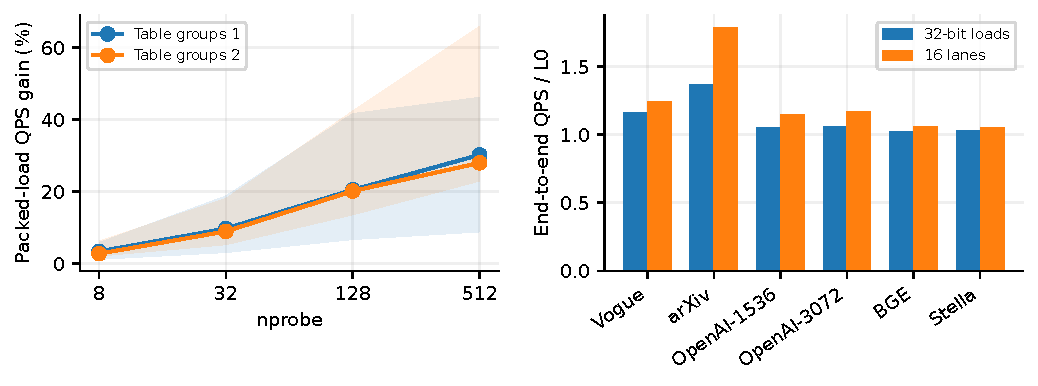
\includegraphics[width=\linewidth]{ch7/packing_refinement.pdf}
\caption{打包访存与精排对照。左：各查找表分组和探针数下，六个数据集打包加载 QPS 增益的中位数，阴影为最小值至最大值。右：128 探针及各数据集普通预算下，仅改变加载和使用 16 个 lane 的实测端到端收益。两个子图来自不同实验组。}
\label{fig:7-packing-refinement}
\end{figure}

\begin{table}[tbp]
\centering
\caption{128 探针下的精排结果。除最后一列为剖析得到的精排内核加速比外，其余比值均为相对 L0 的配对端到端收益。不能将内核加速比与应用整体加速比混用。}
\label{tab:7-refinement}
\small\setlength{\tabcolsep}{4pt}
% Generated by scripts/build_zh_tables.py; numeric rows reuse English tables.
\begin{tabular}{@{}lrrrr@{}}
\toprule
数据集 & $\alpha$ & L1/L0 吞吐比 & L16/L0 吞吐比 & 内核加速比 \\
\midrule
arXiv & 100 & 1.368 & 1.789 & 5.97 \\
BGE & 32 & 1.026 & 1.062 & 1.97 \\
OpenAI-1536 & 8 & 1.055 & 1.145 & 3.34 \\
OpenAI-3072 & 4 & 1.063 & 1.171 & 8.81 \\
Stella & 16 & 1.030 & 1.053 & 2.66 \\
Vogue & 64 & 1.161 & 1.240 & 3.72 \\
\bottomrule
\end{tabular}

\end{table}

在被测用例中，仅改变加载的对照与 L0 逐位一致，但已使 arXiv 吞吐量提高至 $1.368\times$。lane 协作进一步缩短了精排时间。在 arXiv 的 $\alpha=100$ 配置上，精排内核由 4,277.5 降至 716.8\,$\mu$s，即 $5.97\times$ 的内核加速，但整体吞吐量只提高至 $1.789\times$。OpenAI-3072 的精排内核加速为 $8.81\times$，整体吞吐量则为 $1.171\times$。这与 Amdahl 定律一致：加速一个较小阶段，并不能消除路由、筛选、最终选择或传输的成本。这也说明了随后扫描与探针实验的动机——继续处理剩余工作。

定量 Amdahl 检验使用基线精排内核时间占主机到主机基线延迟的比例 $f$，以及内核加速比 $s$；若其余耗时不变，整体估计为 $1/(1-f+f/s)$。arXiv 和 OpenAI-3072 的比例约为 0.529 和 0.168，对应估计 $1.787\times$ 和 $1.175\times$，接近实测 $1.789\times$ 和 $1.171\times$。它结合了单独的内核剖析与墙钟测量，只是机制解释的估计。

协作归约改变了浮点加法顺序。被测多 lane 变体的距离差异很小，最大报告相对误差约为 $1.6\times10^{-6}$，但排序边界附近偶有结果变化。因此，证据支持的是数值接近、且具有实测端到端收益的评分，而不是无条件的逐位等价。Sanitizer 检查在较小查询子集上覆盖了记录中的精排和 top-$k$ 内核；这些是有用的实现检查，并不是对任意输入的证明。

\section{全局 top-c、共享界与探针选择的正确性及消融}
\label{sec:7-4}

本节先回答 RQ2 的正确性部分，再考察分组扫描、阈值共享和基数探针选择的成本。

\subsection{先验证全局主码选择，再讨论性能}

并行扫描实验处理了一个仅靠召回率无法评估的正确性要求：将同一查询的候选分配给多个线程块后，必须保持全局主码 top-$c$。如果每块只保留 $c/\gscan$ 个候选，候选质量集中的分组可能丢弃本应进入全局结果的候选。JHQ 的分组扫描路径改为每组最多保留 $c$ 个候选，再合并局部列表。选择使用完整排序键 $(\primarydist,\mathrm{position})$，以位置确定性地打破主码距离并列。

局部保留规则有直接的正确性解释。一个属于全局 top-$c$ 的候选，在整个候选集合中排在它之前的键少于 $c$ 个，那么在自身所在分组中也一定少于 $c$ 个。因此，它必然出现在该组的局部 top-$c$ 中。对这些局部列表的并集使用相同全序选取 top-$c$，即可恢复全局 top-$c$。这一结论仅针对已访问候选上的主码评分；它不会使 IVF 路由变成精确搜索，不会将主码评分变成原始向量距离，也不会使最终 ANN 答案成为精确最近邻结果。

分组扫描检查覆盖四个工作负载、批大小 8/32/256/1,000，以及分组数 1/2/4/8，共计 64 个比较。记录显示，相对原始单线程块路径，没有非并列情况下的主码选择差异，所比较主码距离的变化为零，而且每条实际使用查询的最终 top-10 标识符与距离逐位一致。原始路径只按距离排序，因此在主码截断边界发生并列时，可能选中不同成员；这并不违反新完整键的规范。在这一特定实验中，这些差异也未改变最终输出。

实际使用的查询数需要单独说明。测试程序只提交完整批次：从 1,000 条查询池中，批大小 32 使用 992 条，批大小 256 使用 768 条，而批大小 8 和 1,000 均使用全部 1,000 条。因此，正确性计数与计时样本随批大小而变化，不能把每一行都描述为相同的 1,000 查询测试。记录中的 memcheck、racecheck 和 synccheck 还对更小子集及指定扫描、合并内核提供了额外检查。

\subsection{共享界保持选择目标不变}

保留完整局部 top-$c$ 是安全的，但成本可能很高。在共享界组件（v63）中，同一查询的各组通过相同完整排序键发布共享界。一旦某组已确定有 $c$ 个键不大于该界，比该界更差的候选就不可能进入全局 top-$c$。过时、较宽松的界可能接纳更多候选，但不会因此错误地排除更优候选。这要求发布的界有足够数量的有效候选作为依据，并且原子更新保持完整键的顺序；仅有近似距离阈值，无法建立相同的并列处理语义。

实现仍会先为每个扫描候选计算完整主码评分，再决定是否接纳。共享界减少的是选择、压缩整理、排序与后续合并工作；它不会剪去主码距离计算，也不会避免读取所有被拒绝候选的主码。解释扫描阶段加速时，必须明确这一范围：扫描阶段变快，并不一定意味着计算了更少距离。

共享界检查，在四个工作负载与四种批大小上，将共享界的 2/4/8 组路径与相应独立界路径比较。48 个比较全部报告主码 top-$c$ 和最终输出一致。五轮配对吞吐量相对独立界约为 $0.994$--$1.562\times$。因此，共享界能显著帮助部分高成本配置，但并非处处更快。在 arXiv 的 $\alpha=200$、批大小 1,000、八组配置上，同一次配对剖析中，合并成本约由 2,629 降至 471\,$\mu$s，扫描则由 7,968 降至 5,513\,$\mu$s。结果支持减少过量中间工作，而不是“扫描分组越多越好”。

另一种未采用的方案是分配更小的静态局部配额。先导工作负载的分布测量显示，第一候选组包含 46--81\% 的全局保留候选。等额配额会经常需要正确性回退；即使校准不等额配额，主导分组仍处于关键路径。这些观测促成了精确共享界设计，但它们只是这些工作负载上的先导测量，不能证明所有可能的配额策略都更差。

\subsection{精确探针选择与流水线一致性的边界}

当筛选变快后，IVF 探针选择在小批次时间中的占比会提高。基数探针原语（v69）改变了选取最小质心评分的实现，同时保留 FP32 评分。其合成检查覆盖 1,792 个用例，失败数为零。在真实 arXiv、Vogue 和 OpenAI-3072 工作负载上，检查发现全部 1,000 条查询的探针标识符相同，主码 top-$c$ 位置与距离也相同。这比“召回率数字没有变化”更具体，因为它直接检查了路由和筛选输出。

\begin{table}[tbp]
\centering
\caption{精确 FP32 探针选择改动的 v69/v65 端到端吞吐量比。每个工作负载—批大小比较中，每个二进制程序共计时十轮，采用交替运行。大于一表示 v69 更快。}
\label{tab:7-probe}
\small
% Generated by scripts/build_zh_tables.py; numeric rows reuse English tables.
\begin{tabular}{@{}lrrrr@{}}
\toprule
数据集 & 批大小 8 & 32 & 256 & 1,000 \\
\midrule
arXiv & 1.074 & 1.063 & 1.035 & 1.034 \\
Vogue & 1.109 & 1.103 & 1.052 & 1.041 \\
OpenAI-3072 & 1.167 & 1.117 & 1.055 & 1.050 \\
\bottomrule
\end{tabular}

\end{table}

\Cref{tab:7-probe} 显示端到端吞吐量提高至 $1.034$--$1.167\times$。批大小为 8 时，剖析得到的探针阶段在 arXiv 上从 56.5 降至 22.6\,$\mu$s，在 Vogue 上从 52.7 降至 14.7\,$\mu$s，在 OpenAI-3072 上从 77.8 降至 16.7\,$\mu$s。大批次下，未修改阶段占整体耗时比例更高，因此整体收益较小符合预期。这些是各自实验组内部的比值，不能把它们与前面的 v62 或精排收益相乘，仿佛所有测量都共享同一个基线。

Vogue 区分了探针原语与跨进程流水线可复现性。在一组、批大小 8 的测试中，两种二进制的探针/主码 dump 对全部 1,000 条查询逐字节相同，但最终召回率为 0.9642 与 0.9644。同一个基线二进制也从一致性运行中的 0.9642，变成之后两次计时运行中的 0.9644。因此，观察到的变化并不需要探针改动才能发生；在 dump 控制的用例中，它出现在已记录主码选择边界之后。残差表示、输入和评分计算仍是可能来源，根因尚未确定。在各被检进程内部，调度与单线程块输出仍逐位一致。附录~\ref{app:reproducibility}明确了 dump 的覆盖范围，避免将其当作对每条计时路径的检查。

最后，可选的 v70 FP16 实验属于另一项近似。在 arXiv 的 936/1,000 条、Vogue 的 979/1,000 条、OpenAI-3072 的 998/1,000 条查询上，其探针集合与 FP32 完全相同，平均集合重叠率很高。但高重叠率和很小的召回率变化，并不能使该原语变成精确操作。这些结果不纳入主要 E1 前沿，也不纳入精确探针选择结论。

\section{留出查询上的预算质量、吞吐量与回本}
\label{sec:7-5}

RQ3 考察相对可信固定预算的质量和摊销成本。因此，比较同时包含沿用的 $\alpha=100$ 与更强的统一固定对照 $\alpha=64$。

\subsection{无标签选择与使用标签的诊断性 oracle}

预算实验在每个数据集—探针数组合中固定一个训练好的索引，比较固定预算、抽样校准、全校准池校准、同样本枚举与离线 oracle。六个数据集均测试 128 和 512 探针。偶数下标查询组成 500 条校准池；奇数下标查询组成互不重叠的 500 条留出池，Stella 例外，留出池为 499 条。从校准池中使用固定随机种子抽取 $S\in\{32,64,128\}$ 条查询，每种大小重复抽取 64 次；单次抽样内不放回。重复抽样使用的是同一个有限查询池，并不等于对未来工作负载漂移进行 64 次独立采样。

降序预算网格为 $A=(200,100,64,32,16,8,4,2)$。校准将候选预算的 top-10 标识符集合与 $\alpha_{\max}=200$ 的参考结果比较。对于样本 $\mathcal Q_S$，接受统计量为
\begin{equation}
 D_S(\alpha)=\sum_{q\in\mathcal Q_S}
 \left(10-|\mathcal R_\alpha(q)\cap\mathcal R_{200}(q)|\right),
 \qquad D_S(\alpha)\leq 1.
 \label{eq:7-agreement}
\end{equation}
允许的是整个样本合计一个结果槽位不一致，而不是每条查询允许一个，也不是基于 ground truth 的召回率容差。实际规则不接收标签。参考结果本身也是近似结果，因此完全一致也可能复制其错误。

离线 oracle 的作用不同。它查看八个固定预算在留出池上的召回率后，在距最佳实测留出召回率不超过 $10^{-3}$ 的配置中选择最快者。这是诊断性比较标准，不是可直接部署的无标签决策。“全校准池”同样表示在全部 500 条校准查询上应用同一校准搜索，而不是利用留出标签枚举所有预算。这些区分避免将“选到与 oracle 相同预算”误解为质量保证。

\subsection{预算质量与抽样风险}

\Cref{tab:7-budget-quality} 给出了 $S=128$ 的结果。十二个单元中，所选预算的中位数有十个与 oracle 预算一致；不一致的两个是 arXiv 的 128 探针配置和 OpenAI-3072 的 512 探针配置。所选预算跨越 4--200，显示出明显的工作负载依赖。然而，预算中位数与平均召回率描述的是抽样总体的不同方面，二者不一定对应某一个配置的性能。此外，表中平均召回率由日志打印的最佳召回率减去打印的平均损失重构，所以保留到四位小数的值是近似值。

\begin{table}[tbp]
\centering
\caption{$S=128$ 时的留出质量。规则的 $\alpha$ 是 64 次抽样的中位数，oracle 的 $\alpha$ 使用留出标签。$\overline R_{\rm rule}$ 是重构的平均召回率。“超标”统计相对最佳被测留出召回率损失 $>10^{-3}$ 的抽样次数；$L_{95}$ 是日志采用较低次序统计量得到的 95 分位损失估计。$R_{100}$ 是固定预算召回率。}
\label{tab:7-budget-quality}
\small\setlength{\tabcolsep}{3pt}
% Generated by scripts/build_zh_tables.py; numeric rows reuse English tables.
\begin{tabular}{@{}lrrrrrr@{}}
\toprule
数据集 & 探针数 & $\alpha$：规则/oracle & $R_{100}$ & $\overline{R}_{\rm rule}$ & 超标 & $L_{95}$ \\
\midrule
Vogue & 128 & 64 / 64 & 0.9680 & 0.9677 & 5/64 & 0.0022 \\
arXiv & 128 & 100 / 200 & 0.9748 & 0.9751 & 40/64 & 0.0024 \\
OpenAI-1536 & 128 & 8 / 8 & 0.9280 & 0.9279 & 4/64 & 0.0000 \\
OpenAI-3072 & 128 & 4 / 4 & 0.9252 & 0.9252 & 0/64 & 0.0000 \\
BGE & 128 & 32 / 32 & 0.9198 & 0.9190 & 1/64 & 0.0008 \\
Stella & 128 & 16 / 16 & 0.9892 & 0.9884 & 6/64 & 0.0030 \\
Vogue & 512 & 64 / 64 & 0.9916 & 0.9915 & 2/64 & 0.0002 \\
arXiv & 512 & 200 / 200 & 0.9878 & 0.9885 & 32/64 & 0.0016 \\
OpenAI-1536 & 512 & 8 / 8 & 0.9740 & 0.9738 & 4/64 & 0.0000 \\
OpenAI-3072 & 512 & 4 / 8 & 0.9704 & 0.9702 & 0/64 & 0.0002 \\
BGE & 512 & 64 / 64 & 0.9670 & 0.9661 & 24/64 & 0.0014 \\
Stella & 512 & 16 / 16 & 0.9954 & 0.9945 & 7/64 & 0.0030 \\
\bottomrule
\end{tabular}

\end{table}

一个重要反例是 arXiv。在 128 探针下，即使平均损失仅为 0.0009，仍有 40/64 次抽样的召回率损失超过 $10^{-3}$；512 探针下有 32/64 次超标。BGE 的 512 探针配置有 24/64 次超标，95 分位损失为 0.0014。Stella 超标次数较少，但两个探针数下的 95 分位损失均为 0.0030。因此，平均质量、超标频率与尾部损失幅度必须一起看。OpenAI-3072 在这些抽样中未观察到超标，这支持其在当前查询池上的有利表现，却不是对未见查询的零风险保证。

对于数量较少的抽样，分位数约定也很重要。测试程序报告排序损失中从零起算的 $\lfloor0.95(64-1)\rfloor=59$ 项，而不是在次序统计量之间插值。因此，可能同时存在四个非零尾部损失，而打印的 $L_{95}=0$，OpenAI-1536 就是如此。表格保留日志统计量与准确超标次数；该列为零不等于所有抽样都没有损失。

\begin{figure}[tbp]
\centering
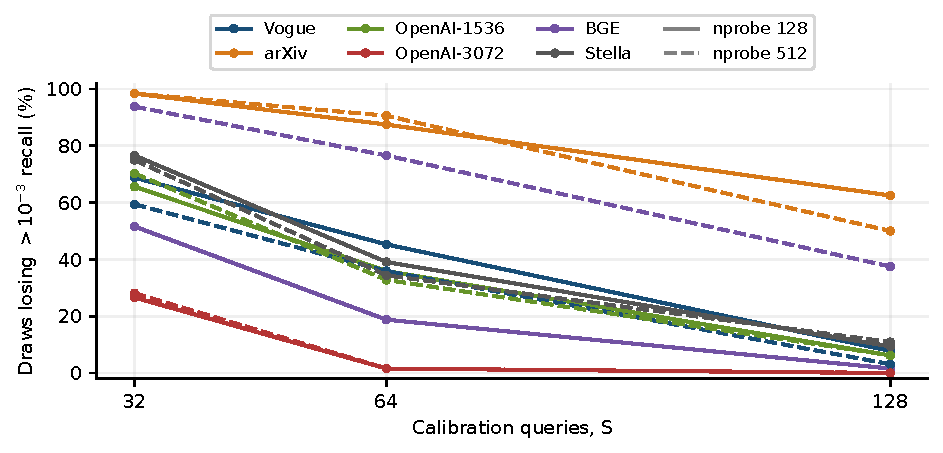
\includegraphics[width=0.82\linewidth]{ch7/budget_risk.pdf}
\caption{不同样本大小下的留出风险。纵轴为相对最佳被测预算，留出召回率损失超过 $10^{-3}$ 的校准抽样百分比。由于\cref{eq:7-agreement}始终保持阈值一，增加 $S$ 也收紧了允许的槽位不一致比例。}
\label{fig:7-budget-risk}
\end{figure}

\Cref{fig:7-budget-risk} 显示了样本大小的影响。更大的样本通常使选择更保守，但同时收紧了归一化允许量 $1/(10S)$。在全部 2,304 次抽样（$12\times3\times64$）中，同样本枚举与二分搜索一致，而打印日志显示枚举耗时为其 1.75--2.01 倍。

被测默认路径执行精确主码 top-$c$，最终 top-$k$ 遍历全部 $c$ 个精排候选，并按 ID 打破并列。有损的 \texttt{K\_LOCAL=4} 保留路径是设置 \texttt{JHQ\_EXACT\_TOPCK=0} 才启用的替代路径，并不是本预算实验单调性限制的原因。在评分固定、采用共同全序并列规则时，精确主码选择得到嵌套候选集，因此抽样一致性准则满足单调性。剩余限制是一块路径在截断并列处只比较距离，以及批大小会决定使用单线程块还是按完整键排序的分组扫描。因此，小校准批次和留出查询批次可能采用不同执行路径。枚举一致验证了这个网格上的抽样决策，并不保证留出召回率，也不保证跨路径无条件嵌套。

固定预算也并不完美。\Cref{tab:7-fixed-budget} 按诊断性质量目标评估了全部八个固定选项。固定 $\alpha=100$ 在十二个单元中有十个达标；$\alpha=200$ 全部达标，但可能牺牲较多吞吐量。全校准池校准也不等于 oracle：在 Vogue 两个探针数下，它均选择 100，而 oracle 选择 64。即使增加校准样本，基于输出一致性的选择与“质量约束下最快”的选择仍解决不同问题。全校准池耗时为 9.5--60.3\,ms。在这十二个单元中，$\alpha=200$ 达到最高实测召回率，因此作为高预算覆盖对照；12/12 达标不是独立的质量保证。网格中的吞吐量也并非严格单调：例如，OpenAI-3072 在 128 探针下，$\alpha=2$ 为 128.7 kQPS，$\alpha=4$ 为 145.0 kQPS。三次计时无法区分时间波动与配置相关执行成本，所以本章不为该倒置认定机制。

\begin{table}[tbp]
\centering
\caption{十二个留出单元上的固定预算对照。达标表示按打印精度，距最佳被测召回率不超过 $10^{-3}$。最大召回率损失使用全部单元，QPS 差额只统计该预算达标的单元。横线表示没有达标单元。}
\label{tab:7-fixed-budget}
\small
% Generated by scripts/build_zh_tables.py; numeric rows reuse English tables.
\begin{tabular}{@{}rrrr@{}}
\toprule
$\alpha$ & 达标单元 & 最大召回率损失 & 达标单元最大 QPS 差额 \\
\midrule
2 & 0/12 & 0.3100 & -- \\
4 & 2/12 & 0.1774 & 2.3\% \\
8 & 4/12 & 0.0930 & 2.1\% \\
16 & 6/12 & 0.0408 & 4.4\% \\
32 & 7/12 & 0.0170 & 9.1\% \\
64 & 10/12 & 0.0050 & 26.6\% \\
100 & 10/12 & 0.0016 & 40.9\% \\
200 & 12/12 & 0.0000 & 57.1\% \\
\bottomrule
\end{tabular}

\end{table}

\subsection{估计吞吐量与校准经济性}

与 E1 不同，这组实验在预热后，对每个固定配置进行三次搜索计时。规则报告的 QPS 是 64 次抽样所选配置的已有实测 QPS 的算术平均，而不是对一个重复执行“校准—搜索”的服务进行新计时。当 $S=128$ 时，这一所选配置吞吐量估计在十个单元中优于固定 $\alpha=100$，比值为 $1.028$--$1.691\times$。arXiv 的比值则为 0.908 和 0.917：平均召回率提高，但吞吐量降低。这两个单元无法通过吞吐量收益回本。

更强的 $\alpha=64$ 对照缩小了整体收益：所选配置的平均 QPS 在 9/12 个单元中胜出，几何平均比值为 $1.054\times$，范围为 $0.821$--$1.367\times$。Vogue 几乎不变；BGE 的 512 探针配置只提高 0.6\%；OpenAI 的收益范围为 $1.052$--$1.367\times$。固定 64 和固定 100 都在 10/12 个单元达标，失败的都是两个 arXiv 单元。校准的价值是适应不同精排需求，而不是始终击败已经合理的固定预算。

arXiv 的超标是相对最佳被测留出召回率，不是相对默认配置。固定 100 在 128 和 512 探针下本来分别损失 0.0012 和 0.0016，而抽样平均损失在两个单元均为 0.0009。因此，即使部分抽样超过相对 oracle 的目标，平均质量仍比默认配置更好。

\begin{table}[tbp]
\centering
\caption{校准经济性，$S=128$。速率单位为 kQPS，规则速率为所选配置平均 QPS。比值分别相对固定 100 与固定 64。最后一列回本相对固定 100，使用 500 条查询，Stella 为 499；“不回本”表示没有吞吐量回本。}
\label{tab:7-budget-cost}
\footnotesize\setlength{\tabcolsep}{3pt}
% Generated by scripts/build_zh_tables.py; numeric rows reuse English tables.
\begin{tabular}{@{}lrrrrrrrr@{}}
\toprule
数据集 & 探针数 & $Q_{100}$ & $\overline Q_{\rm rule}$ & 相对 100 & 相对 64 & 校准 ms & 回本批数 & \shortstack{固定 100\\质量} \\
\midrule
Vogue & 128 & 202.9 & 224.4 & 1.106 & 1.004 & 4.0 & 17.0 & 达标 \\
arXiv & 128 & 207.9 & 188.8 & 0.908 & 0.821 & 4.2 & 不回本 & 未达标 \\
OpenAI-1536 & 128 & 167.5 & 268.5 & 1.603 & 1.367 & 3.9 & 3.5 & 达标 \\
OpenAI-3072 & 128 & 85.7 & 145.0 & 1.691 & 1.230 & 5.7 & 2.4 & 达标 \\
BGE & 128 & 116.2 & 131.2 & 1.130 & 1.051 & 6.5 & 13.2 & 达标 \\
Stella & 128 & 95.7 & 110.3 & 1.153 & 1.087 & 7.5 & 10.8 & 达标 \\
Vogue & 512 & 100.1 & 102.9 & 1.028 & 0.996 & 7.5 & 55.4 & 达标 \\
arXiv & 512 & 83.1 & 76.2 & 0.917 & 0.870 & 9.7 & 不回本 & 未达标 \\
OpenAI-1536 & 512 & 86.6 & 115.0 & 1.327 & 1.268 & 8.8 & 6.2 & 达标 \\
OpenAI-3072 & 512 & 42.8 & 52.1 & 1.219 & 1.052 & 13.1 & 6.2 & 达标 \\
BGE & 512 & 49.2 & 51.1 & 1.039 & 1.006 & 15.8 & 41.2 & 达标 \\
Stella & 512 & 34.6 & 36.0 & 1.041 & 1.028 & 21.3 & 37.1 & 达标 \\
\bottomrule
\end{tabular}

\end{table}

日志中的校准成本为 3.9--21.3\,ms。它包含参考搜索与输出一致性检查，以及测量搜索调用内包含的相关设置，但不包含将抽样向量收集到输入缓冲区的操作。对于相同大小的后续批次，定义
\begin{equation}
 B^*=\frac{T_{\rm cal}}{T_{100}-T_{\rm rule}},\qquad
 T_{\rm rule}<T_{100}.
 \label{eq:7-payback}
\end{equation}
使用 $T_{\rm rule}\approx n/\overline Q_{\rm rule}$ 得到\cref{tab:7-budget-cost}中的估计：有利单元相对固定 100 约需 2.4--55.4 个留出池大小的后续批次。相对固定 64，九个有利单元约需 5.7--404.3 批，Vogue 的 512 探针配置没有吞吐量回本。\Cref{fig:7-budget-payback}对两个对照都使用实际留出查询数。

\begin{figure}[tbp]
\centering
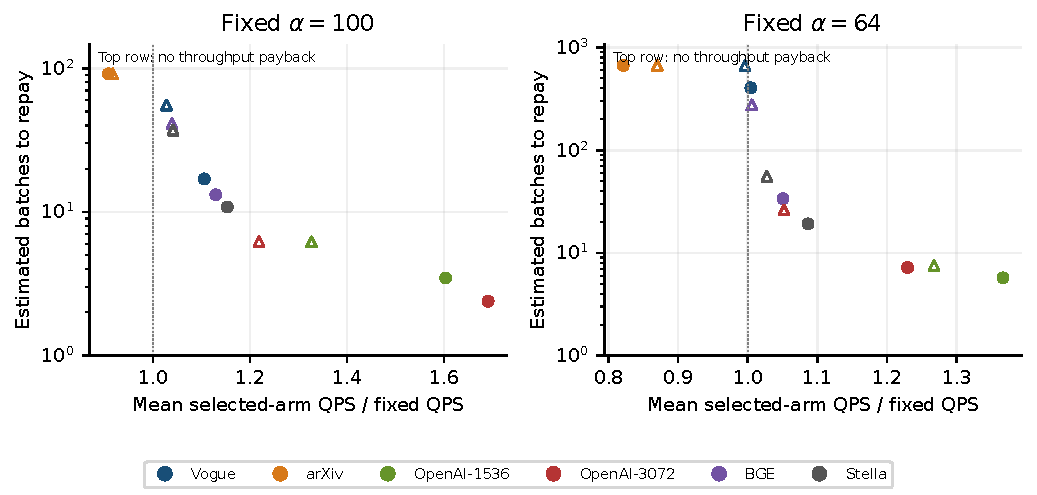
\includegraphics[width=\linewidth]{ch7/budget_payback.pdf}
\caption{相对固定预算 100 和 64 的校准回本估计。实心圆表示 128 探针，空心三角表示 512 探针；顶行点没有吞吐量回本。估计对所选配置平均 QPS 取倒数，使用 500 条查询，Stella 为 499。}
\label{fig:7-budget-payback}
\end{figure}

这种计算偏乐观。一般而言，$1/\mathbb E[Q]\leq\mathbb E[1/Q]$，所以当不同校准抽样选择了速率不同的配置时，对平均 QPS 取倒数会低估平均执行时间。样本收集、未来查询漂移与重新校准开销也会影响摊销。对于长期稳定的工作负载，复用策略可能带来收益；短任务或变化的查询总体则未必如此。当前实验没有测量漂移检测，也没有测量生产环境中的重新校准计划。

作为历史比较，较早的标量精排实现（v57）在 10/12 个单元中报告相对固定 100 的 $1.054$--$2.773\times$ 收益，校准耗时为 5.2--30.8\,ms。较新的 lane 精排流水线收益更小，与可节省精排时间减少的解释相容。两次运行共享预算协议和网格，但跨实验比较并未隔离证明精排是变化的唯一原因。

\section{批大小、扫描组调度与工作负载偏斜}
\label{sec:7-6}

本节回答 RQ2 的性能区间问题：何时额外扫描组提供有价值的并行度，何时额外工作成为主导。

\subsection{并行度与重复选择工作的权衡}

扫描实验揭示了两种执行区间。每条查询使用一个线程块时，批大小 8 只在具有 170 个 SM 的设备上提供八个线程块。划分候选能增加可用线程块并行度。在 v62 实验中，批大小 8 使用八组后，端到端吞吐量为原来的 $2.06$--$2.76\times$。剖析给出了阶段解释：arXiv 扫描约从 849 降至 216\,$\mu$s，Vogue 从 1,059 降至 246\,$\mu$s，OpenAI-3072 从 728 降至 155\,$\mu$s。额外合并分别约需 16.7、9.1 和 3.7\,$\mu$s。即使支付合并成本，净节省仍很大。

批大小为 1,000 时，独立查询已足以提供较多线程块。增加分组会重复搬入查找表、接纳局部候选并排序，还产生额外合并流量。对于 arXiv 的 $\alpha=200$ 配置，不共享界的 v62 路径可能降至单线程块基线的约 $0.46\times$。全批次剖析显示，$\alpha=100$ 的扫描从 2,922 增至 6,079\,$\mu$s，$\alpha=200$ 从 3,530 增至 7,652\,$\mu$s，后者还增加了 2,624\,$\mu$s 合并时间。这一反向结果对设计至关重要：并行拆分能够解决并发不足，但当并发已经充足时，它引入的额外工作可能成为主导。共享界减少了这些额外工作，却没有消除执行区间的变化。

\begin{figure}[tbp]
\centering
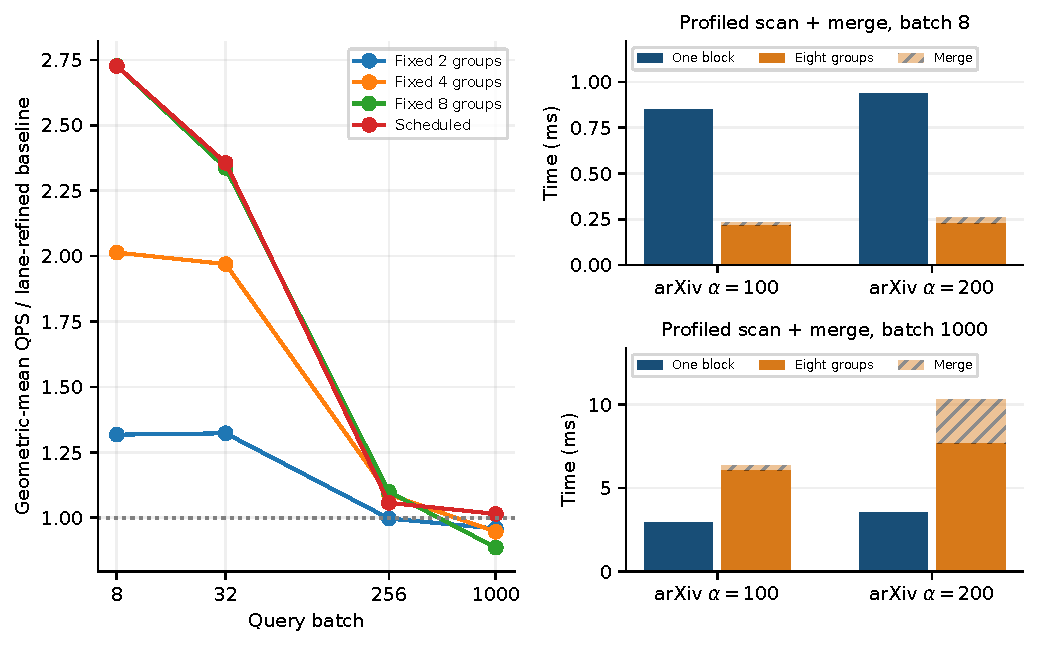
\includegraphics[width=\linewidth]{ch7/batch_execution.pdf}
\caption{执行区间。左：共享界固定组数与调度执行，相对 lane 精排单线程块基线的吞吐量比，较小批次有 13 个单元，批大小 1,000 有 11 个。右：arXiv 预算 100 和 200 在批大小 8 与 1,000 下的配对扫描、合并剖析；斜线表示合并时间。右侧来自独立界扫描实验，用于解释一项成本，不代表调度器全部收益。}
\label{fig:7-batch}
\end{figure}

\subsection{在更多配置上评估预先固定的规则}

集成批调度器（v65）根据批大小、线程块大小以及工作负载偏斜估计选择扫描组数。填充规则将潜在线程常驻数量与设备线程容量的固定 0.6 比例关联；偏斜规则则在每条查询候选数的变异系数至少为 0.3 时，要求至少使用四组。最终取两条规则建议的较大组数；一组情况映射到原始单线程块扫描。偏斜统计只估计一次，使用 512 个数据库向量作为伪查询，不使用 ground-truth 标签或被测查询池。规则常数在四个工作负载配置上确定，之后才测量额外配置。

\begin{table}[tbp]
\centering
\caption{集成执行相对 v61 L16 的收益。每项先计算单元内五轮配对加速比的中位数，再跨单元取几何平均。“留出配置”排除了设置规则时使用的四个配置，指的是未用于设定规则的配置，不是预算实验中的留出查询划分。}
\label{tab:7-scheduling}
\small\setlength{\tabcolsep}{4pt}
% Generated by scripts/build_zh_tables.py; numeric rows reuse English tables.
\begin{tabular}{@{}rrrrrrr@{}}
\toprule
批大小 & 单元数 & $g_s=2$ & $g_s=4$ & $g_s=8$ & 调度 & 留出配置 \\
\midrule
8 & 13 & 1.318 & 2.014 & 2.728 & 2.727 & 2.930 \\
32 & 13 & 1.323 & 1.970 & 2.337 & 2.356 & 2.560 \\
256 & 13 & 0.997 & 1.090 & 1.099 & 1.057 & 1.041 \\
1000 & 11 & 0.959 & 0.947 & 0.886 & 1.015 & 1.012 \\
\bottomrule
\end{tabular}

\end{table}

\Cref{tab:7-scheduling} 从原始计时数组重新计算结果。批大小为 8、32、256 和 1,000 时，调度收益的几何平均分别为 $2.727\times$、$2.356\times$、$1.057\times$ 和 $1.015\times$。前三种批大小有十三个配置，其中包含额外的 arXiv 高预算配置；批大小 1,000 只有十一个，因为 Stella 的 999 条查询池无法组成一个完整的 1,000 查询批次。对应的留出配置子集分别含九个和七个配置。因此，将这些均值连接起来的图总结的是运行区间，而不是完全平衡的重复测量总体。

固定八组在批大小 8 时的均值接近调度结果，但在批大小 1,000 时降至 $0.886\times$。调度大体保留了小批次收益，并避免上述大批次损失。不过，它仍是启发式规则，不是 oracle。批大小 256 时，在一个 BGE 配置上，“最佳固定吞吐量 / 调度吞吐量”的最差比值为 1.217。候选数 CV 无法描述列表遍历、选择或合并的全部成本。这一失败表明所选特征存在局限，并不说明执行调度没有必要。

Vogue 说明仅看批大小是不够的。其候选数 CV 实测约为 0.51，而原始其他工作负载约为 0.08--0.11；其最重查询的候选数约为均值的 2.2 倍。划分候选能缩短慢查询，而该查询原本可能决定整个同步批次的完成时间。这解释了为何 Vogue 在较大批次下仍可能受益于多组执行，不过这些 CV 观测仍属于工作负载证据，并不是对偏斜作用的普遍因果隔离。

最后，正确性检查独立于计时。在 250 个变体/配置比较、234,320 次逐查询比较中，集成实验未发现非并列主码选择差异，也未发现最终标识符集合差异。在并列情况下，最终顺序可能不同，因而不能将整个实验描述为无条件逐位一致。吞吐量结果针对顺序同步提交，不足以建立开放到达过程下的尾延迟表现。

\section{冷构建、常驻显存与已验证规模}
\label{sec:7-7}

通过冷构建、常驻显存与已完成的大数据集搜索评估 RQ1；E1 显存比较也为 RQ4 提供依据。

\subsection{冷构建与生命周期边界}

主要搜索扫描复用了已训练状态缓存。加载该状态并添加向量不属于冷构建。独立日志明确在训练状态缓存为空时训练，然后编码并添加数据库；\cref{tab:7-build-memory}给出这些记录中的训练与添加时间。合计耗时从 OpenAI-1536 的约 1.01\,s 到 Stella 的 10.40\,s。Stella 的训练为 3.74\,s、添加为 6.67\,s，也说明不能仅凭另一个阶段或数据集规模可靠推断某个阶段的成本。

\begin{table}[tbp]
\centering
\caption{JHQ 冷构建与单独测量的常驻显存。训练和添加来自每个数据集的一次已记录冷构建；显存来自 v71 两组、128 探针、$\alpha=100$ 的运行，包含上下文与工作区。“残差占比”表示模型计算的残差码占实测已用总量的比例，而不是每次查询读取的比例。}
\label{tab:7-build-memory}
\small\setlength{\tabcolsep}{3pt}
% Generated by scripts/build_zh_tables.py; numeric rows reuse English tables.
\begin{tabular}{@{}lrrrrrr@{}}
\toprule
数据集 & 训练 s & 添加 s & 合计 s & 已用 GiB & 原始 GiB & 残差占比 \\
\midrule
Vogue & 1.06 & 0.27 & 1.33 & 1.47 & 2.67 & 45.4\% \\
arXiv & 0.59 & 0.52 & 1.10 & 2.58 & 6.45 & 62.5\% \\
OpenAI-1536 & 0.64 & 0.38 & 1.01 & 2.39 & 5.72 & 59.7\% \\
OpenAI-3072 & 1.34 & 0.65 & 1.99 & 4.14 & 11.43 & 69.0\% \\
BGE & 3.75 & 3.67 & 7.42 & 11.93 & 38.50 & 80.7\% \\
Stella & 3.74 & 6.67 & 10.40 & 20.44 & 67.81 & 82.9\% \\
\bottomrule
\end{tabular}

\end{table}

这里的“冷”指已学习索引状态。输入加载器可复用内存映射 FP32 数据；报告的训练加添加区间不包含从存储设备读取原始导出文件。调度器的伪查询校准在添加之后进行，也不计入总量。完整部署生命周期还应考虑数据准备、某些接口未计入的传输、校准、序列化和后续查询时间。这些记录是在明确边界内有价值的构建测量，不是完整端到端数据摄取服务的成本。

比较图同时给出了其他构建配置与这些冷构建记录。每种方法的范围不是等价重复构建的置信区间。训练样本、索引参数与表示不同，而且每个数据集只有一次 JHQ 冷构建记录。对于 RaBitQ，记录中的构建函数与序列化/反序列化分开计时，但基准必须完成该往返后才能搜索。只有将柱形明确标为构建函数时间时，才可以不计这一步；它并不表示直到第一次可用搜索的全部时间。

\begin{figure}[tbp]
\centering
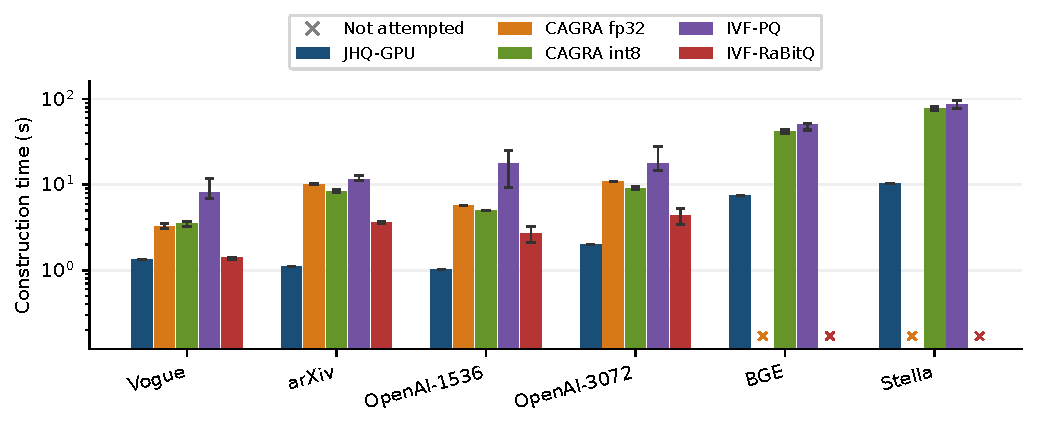
\includegraphics[width=\linewidth]{ch7/construction.pdf}
\caption{包括 CAGRA int8 的已记录构建成本。JHQ 为一次冷训练加添加记录；其他柱形为成功测量的索引配置之间的中位数，误差线表示最小值至最大值。Int8 包含数据集量化；RaBitQ 不包含所需的序列化往返。大数据集缺失的柱形表示未尝试的配置，不代表实测构建失败。纵轴为对数坐标。}
\label{fig:7-build}
\end{figure}

在 Stella 上，CAGRA int8 成功的隔离构建按图出度不同，包含数据集量化后约为 74.55 和 82.45\,s；IVF-PQ 三个配置的实测构建中位数为 86.59\,s。在报告边界内，JHQ 的 10.40\,s 明显更短，但不能据此证明它在所有条件下构建最快，也不能证明后续召回率相同。构建速度、可搜索质量与常驻成本是部署时需要分别考虑的维度。

\subsection{常驻分配与压缩发挥作用的位置}

\Cref{fig:7-memory} 分解常驻显存。标记表示记录时设备已用显存，而不是纯索引分配。堆叠部分用模型计算主码、残差码、修正因子与标识符、质心、每批查找表、候选缓冲区和列表分组临时区。剩余实测分配明确保留为未归因部分；它可能包含运行时上下文、分配器影响以及模型遗漏的分配。将剩余部分全部归给残差码，会高估表示成本。

\begin{figure}[tbp]
\centering
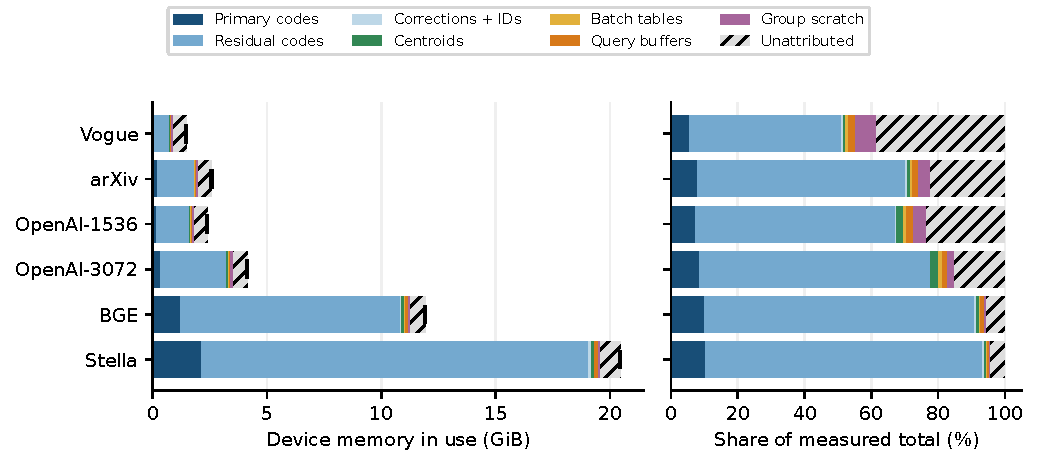
\includegraphics[width=\linewidth]{ch7/memory.pdf}
\caption{两组查找表、128 探针、$\alpha=100$ 下的常驻显存分解。组件大小由模型计算，标记为实测已用总量，斜线区域为未归因部分。总量包含上下文与工作区，未测量构建峰值。}
\label{fig:7-memory}
\end{figure}

在大数据集上，残差码是主要占用：BGE 的已用总量为 11.93\,GiB，其中约 80.7\% 为残差码；Stella 为 20.44\,GiB，其中约 82.9\% 为残差码。仅对应的原始 FP32 向量数组就分别需要 38.50 和 67.81\,GiB。因此，JHQ 通过保留压缩层次表示，使这些已测试的数据能够在单卡常驻搜索。降低 $\alpha$ 会减少每条查询访问、评分的残差码，但不会释放已经存储的残差数组。同样，笛卡尔 LUT 因子化减少的是查询相关查找表存储，不是数据库残差码的精度。

工作区同样重要。在这些 $\alpha=100$ 测量中，报告的列表分组临时区约为 93.8\,MiB，即使实际执行选择单线程块路径，也为批容量 1,024 和最多八组预留。因此，实际组数变小，不意味着分配按比例缩小。另一方面，这些常驻样本没有捕获临时构建峰值。基线测试程序也在测量索引显存之后才初始化部分搜索内存池，因此，不能把构建后的索引增量当作各方法完整进程峰值显存预算。

E1 测量提供了\cref{tab:7-e1-memory}中的独立跨系统视图。从 JHQ 进程总量减去基线测得的 507.2\,MiB 上下文后，约为 CAGRA fp32 索引分配的 0.29--0.39。JHQ 数字包含工作区，CAGRA 数字则是构建时索引增量。这些是参数扫描范围，不是显存匹配的同召回率运行点，也不是相同峰值预算的比较。

\begin{table}[tbp]
\centering
\caption{E1 分配范围。JHQ 为进程总量减去 507.2\,MiB 上下文估计，包含查询工作区；CAGRA fp32 为构建时测量的索引分配。比值范围组合每个数据集的极值。}
\label{tab:7-e1-memory}
\footnotesize\setlength{\tabcolsep}{4pt}
% Generated by scripts/build_zh_tables.py; numeric rows reuse English tables.
\begin{tabular}{@{}lrrr@{}}
\toprule
数据集 & JHQ 净进程 GiB & CAGRA fp32 索引 GiB & 比值范围 \\
\midrule
Vogue & 0.90--1.01 & 2.89--2.91 & 0.31--0.35 \\
arXiv & 2.01--2.19 & 6.84--6.98 & 0.29--0.32 \\
OpenAI-1536 & 1.79--2.33 & 5.95--5.97 & 0.30--0.39 \\
OpenAI-3072 & 3.54--3.82 & 11.67--11.68 & 0.30--0.33 \\
\bottomrule
\end{tabular}

\end{table}

\subsection{大数据集可运行性与竞争区间}

BGE 含 10,091,524 个向量，Stella 含 17,776,615 个向量，均为 1,024 维、32,768 个 IVF 列表。Stella 查询采样自语料库，因此结果描述的是该基准，而不是独立收集的外部查询分布。\Cref{fig:7-large} 包含成功的 CAGRA int8 和 IVF-PQ 测量。对于计算存储需求超过可用设备容量的全精度 CAGRA、RaBitQ 配置和 FP32 暴力搜索，大规模比较没有尝试运行。这些缺项是预先进行的可运行性排除，不是观察到的显存耗尽错误或实测召回率失败。

\begin{figure}[tbp]
\centering
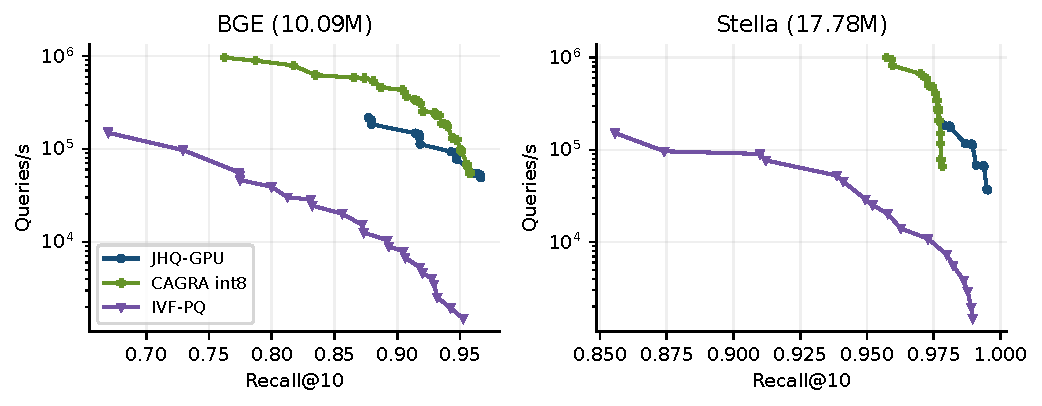
\includegraphics[width=\linewidth]{ch7/large_frontiers.pdf}
\caption{大数据集上的主机到主机前沿，包含 CAGRA int8 成功的隔离重跑。BGE 使用 1,000 条查询，Stella 使用 999 条。曲线端点是已测试网格的终点，不是方法的内在召回率上限。}
\label{fig:7-large}
\end{figure}

成功的隔离重跑显示，CAGRA int8 能在被测配置下装入 Stella。在 BGE 的共同采样目标 0.88/0.90/0.92/0.94/0.95 上，int8 约比 JHQ 快 $1.35$--$2.96\times$；在 int8 的最高实测召回率 0.9579 处，JHQ 插值 QPS 是 int8 的 $1.086\times$。因此，优势在高召回率末端附近反转。BGE/Stella 上，int8 的最高被测召回率为 0.9579/0.9783，JHQ 为 0.9663/0.9952，PQ 为 0.9525/0.9896。

Stella 上一个具体高端比较为：JHQ 在召回率 0.978679 时达到 185.4 kQPS，int8 在 0.978278 时为 66.3 kQPS，速率比为 $2.80\times$，两者召回率略有不同。这是一对明确的实测点，不是统一的匹配召回率优势：JHQ 很多更高召回率区间没有 int8 覆盖，而且其最高召回率点也以吞吐量换取质量。附录~\ref{app:reproducibility}记录修正运行的排除规则与测试程序诊断。

结果证明的是已测试规模和有价值的高召回率区间，而不是任意规模的可扩展性。最大已完成搜索是在单 GPU 上处理 17.78 百万个向量；本章没有多 GPU 实验，没有保持数据分布不变的扩展曲线，也没有接近显卡容量时的构建峰值证明。Stella 搜索使用实际的 999 条查询池。

\section{数值稳健性、异常与召回率归因}
\label{sec:7-8}

稳健性检查界定 RQ2 的精确性声明、RQ3 的风险评估与 RQ4 中较小的跨系统差距。

\subsection{质量分辨率与重复执行}

当 $k=10$、查询数为 1,000 时，多找回一个邻居会使总体 Recall@10 改变 $10^{-4}$；500 条留出查询时，分辨率为 $2\times10^{-4}$。Stella 的 499 查询划分略粗。这种离散分辨率不是不确定性区间，但有助于理解前面的小差异。第四位小数的变化可能只对应一两个结果槽位，而小的平均损失仍可能掩盖若干答案变化较大的查询。

重复计时调用也必须与重复索引构建分开。E1 解析器记录了 369 个标识符确定性标记为 false 的基线运行点：170 个 RaBitQ、80 个 IVF-PQ、68 个 CAGRA int8、50 个 CAGRA fp32，以及一个暴力搜索点。该标记可能包括并列结果的顺序变化，本身不意味着标识符集合变化或输出无效。没有测量点仅因这一标记而被丢弃。原始日志保留首次/末次召回率与集合、顺序诊断。JHQ 没有填写同样的基线标记，因此不能把它缺失该标记当作统一的跨方法确定性测试。较早 E1 报告的 401 使用的是 369 个 A 重复调用标记与 367 个 B 相对 A 不匹配标记的并集；其中 32 个点仅增加后一种标记。B 与 A 不一致是跨协议相等性检查，不等于重复调用 B 不确定。

五轮吞吐量摘要保留了固定构建内部的变化。最小值和最大值是描述性范围，不是置信区间，也不包括训练差异。因此，对两个 LUT 接近平手的例子、或 arXiv 与 RaBitQ 在召回率 0.97 处的小幅差距，不应赋予太大的解释权重。与对应阶段时间减少相匹配、幅度较大且能重复的收益，比单独一处微小前沿移动更能支持执行优化结论。

在各数据集 RaBitQ 配置间，“五轮最大值减最小值 / QPS 中位数”的中位数分别为：Vogue 3.79\%、arXiv 3.34\%、OpenAI-1536 2.87\%、OpenAI-3072 5.25\%。这些描述性波动与 Vogue 小幅领先的量级接近，而不是匹配比值的置信区间。原始调用轨迹也包含长调用，在原本较快的配置中偶有 30--60\,ms 观测。敏感性检验对 1,000 条查询的一次调用，按 $10^6/\operatorname{median}(\text{call latency in ms})$ 重算 QPS，以减小长调用的影响。召回率 0.97 处，得到的 JHQ/RaBitQ 比值为 1.063、0.995、1.118 和 1.100。三个有利方向与 arXiv 接近平手的格局保持，因此结果不只是长调用造成的。

\subsection{精确性必须限定到具体阶段}

几项不同声明必须区分。笛卡尔因子化在代数上保持已表示评分；打包加载保持逻辑编码值；采用完整键的局部保留和合并恢复已访问候选中的精确主码 top-$c$；共享界保持该选择目标；FP32 探针原语通过了合成与真实输入的等价检查。以上任何一项，都不等于在原始向量空间找到了精确最近邻。

lane 归约会改变舍入；主码截断边界的并列可能改变被精排的候选；最终选择对全部保留的精排评分进行精确选择，并按 ID 打破并列；相对原空间邻居的剩余误差可以来自此前阶段或已表示评分。归档中的 Vogue 跨版本差异说明，完整流水线的一致性需要独立检查。类似地，FP16 路由实验表明，几乎不变的平均召回率也不足以证明探针精确等价。因此，主要正确性结论都限定到实际测试过的阶段与输入覆盖。

召回率损失可能来自路由、主码筛选、残差评分或最终选择。增加探针扩大路由覆盖；增加 $\alpha$ 使更多主码候选进入残差评分；二者都不能恢复后续所有近似阶段丢失的信息。预算扫描固定索引和探针配置，直接测量改变保留候选数量的影响，却没有把每个遗漏邻居分解为唯一原因。完整逐查询归因需要在路由、主码保留和精排后分别检查真实邻居覆盖，并对同一候选集使用精确最终选择作为参考。本章所用实验尚未建立这种完整归因，因此不为未测量的损失来源分配百分比。

\subsection{研究发现的适用范围}

\Cref{tab:7-rq-answers} 收束 RQ1--RQ4 的证据链。结果支持少量面向表示的执行模式与工作负载相关精排工作量，并分别提供正确性、速度和质量证据。

\begin{table}[tbp]
\centering
\caption{本章证据支持的四个研究问题答案。}
\label{tab:7-rq-answers}
\small
\begin{tabularx}{\linewidth}{@{}l*{3}{>{\raggedright\arraybackslash}X}@{}}
\toprule
研究问题 & 证据 & 答案 & 边界 \\
\midrule
RQ1 & 冷构建、常驻组件、大规模搜索 & 单卡 17.78M 向量；20.44\,GiB；训练加添加 10.40\,s & 单次冷记录；未测构建峰值或多 GPU 扩展 \\
RQ2 & LUT、精排、扫描、共享界、探针配对测试 & 被测主码选择精确；批大小 8 调度为 $2.727\times$ & 并列与数值路径；全批次收益小得多 \\
RQ3 & 互斥查询划分、固定 64/100、oracle、枚举 & 平均 QPS 相对 64 胜 9/12，相对 100 胜 10/12 & 校准开销；最多 40/64 次相对 oracle 损失超标；未测漂移 \\
RQ4 & 六方法 E1 扫描、匹配召回率、显存 & 0.97 处三个领先，arXiv 接近平手；净分配低于 fp32 CAGRA & int8 在低召回率领先；端点和计时不确定性 \\
\bottomrule
\end{tabularx}
\end{table}

结论适用于平方 L2 的 top-10 搜索、记录查询池与被测 RTX 5090 环境。跨设备行为、变化查询、在线更新与开放到达服务延迟尚未测试。这些边界与正面结果共同呈现，而不是取代正面发现。
